\documentclass{article}

\usepackage{ragged2e}
\usepackage{graphicx}
\usepackage{amsmath}
\usepackage{siunitx}
\usepackage{tabu}
\usepackage{array}

\begin{document}
    
\begin{flushright}
    \noindent
    Rodrigo Becerril Ferreyra\\
    CECS 211 Section 01\\
    Lab 4\\
    2019-09-19--2019-09-24
\end{flushright}

Here is a diagram of the circuit we will be solving:

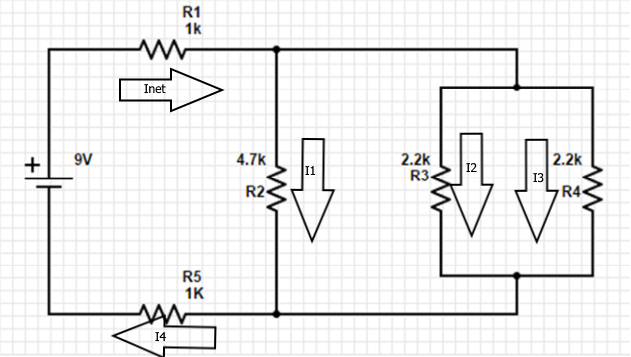
\includegraphics[width=\textwidth]{Diagram.png}

The given values for this circuit are as follows:

\begin{align*}
    V_s &= \SI{9}{\volt}\\
    R_1 &= \SI{1}{\kilo\ohm}\\
    R_2 &= \SI{4.7}{\kilo\ohm}\\
    R_3 = R_4 &= \SI{2.2}{\kilo\ohm}\\
    R_5 &= \SI{1}{\kilo\ohm}
\end{align*}

The equivalent resistance for this circuit can be calculated
as follows:

\begin{align*}
    R_{\text{net}} &= R_1 + ((R_3 \parallel R_4) \parallel R_2) + R_5\\
%    &= R_1 + R_{\text{equ}} + R_5 \\
    &= \SI{1}{\kilo\ohm} + ((\SI{2.2}{\kilo\ohm} \parallel \SI{2.2}{\kilo\ohm}) \parallel \SI{4.7}{\kilo\ohm}) + \SI{1}{\kilo\ohm}\\
    &= \SI{1}{\kilo\ohm} + (\SI{1.1}{\kilo\ohm} \parallel \SI{4.7}{\kilo\ohm}) + \SI{1}{\kilo\ohm}\\
    &= \SI{1}{\kilo\ohm} + \SI{0.891}{\kilo\ohm} + \SI{1}{\kilo\ohm}\\
    &= \SI{2.891}{\kilo\ohm}
\end{align*}

Using Ohm's Law $(V=IR)$, we can find the total current
for the circuit:

\begin{align*}
    I_{\text{net}} &= \frac{V_s}{R_{\text{net}}}\\
    &= \frac{\SI{9}{\volt}}{\SI{2.891}{\kilo\ohm}} = \SI{3.113}{\milli\ampere}
\end{align*}

The amount of current going through each resistor and the
amount of voltage dropped by each resistor can also be
calculated using Ohm's Law.

\begin{center}
\begin{tabular}[c]{r|l}

    $I_{\text{net}}$ & \SI{3.113}{\milli\ampere} \\
    $V_{R_1}$ & $\SI{3.113}{\milli\ampere} \times \SI{1}{\kilo\ohm} = \SI{3.113}{\volt}$ \\
    $V_{R_2}$ & $V_s - (V_{R_1} + V_{R_5}) = \SI{9}{\volt} - (\SI{3.113}{\volt} + \SI{3.113}{\volt}) = \SI{2.774}{\volt}$ \\
    $V_{R_3}$ & $\SI{2.774}{\volt}$ \\
    $V_{R_4}$ & $\SI{2.774}{\volt}$ \\
    $V_{R_5}$ & $\SI{3.113}{\milli\ampere} \times \SI{1}{\kilo\ohm} = \SI{3.113}{\volt}$ \\
    $I_1$ & $\SI{2.774}{\volt} / \SI{4.7}{\kilo\ohm} = \SI{0.590}{\milli\ampere}$ \\
    $I_2$ & $\SI{2.774}{\volt} / \SI{2.2}{\kilo\ohm} = \SI{1.261}{\milli\ampere}$ \\
    $I_3$ & $\SI{2.774}{\volt} / \SI{2.2}{\kilo\ohm} = \SI{1.261}{\milli\ampere}$ \\
    $I_4$ & $\SI{3.113}{\volt} / \SI{1}{\kilo\ohm} = \SI{3.113}{\milli\ampere}$ \\

\end{tabular}
\end{center}

Here are all the values for voltage when simulated in Multisim:

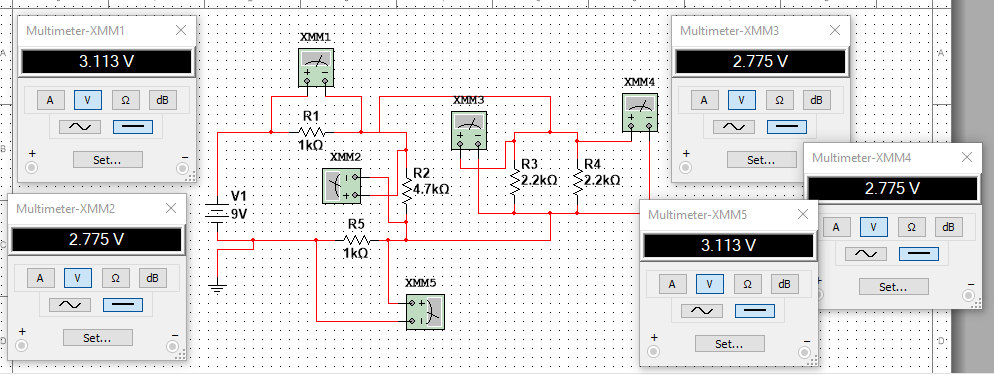
\includegraphics[width=\textwidth]{Lab4Voltage.png}

And here are all the values for current:

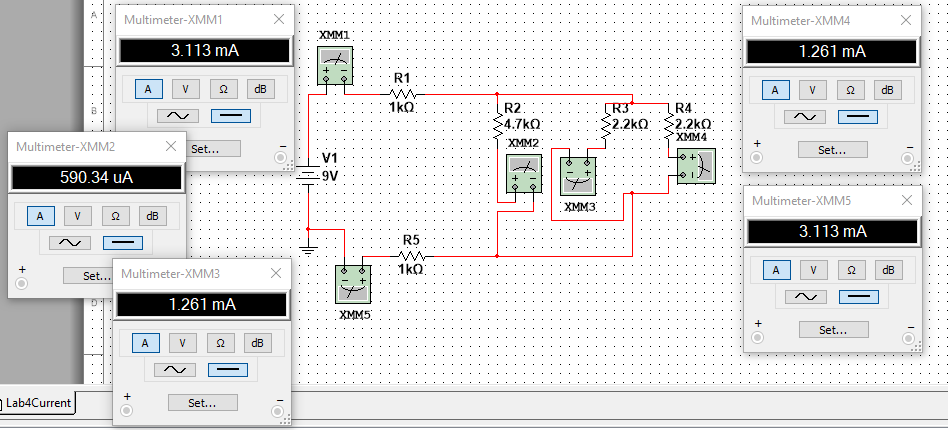
\includegraphics[width=\textwidth]{Lab4Current.png}

\pagebreak

Here is the physical breadboard build of this circuit:

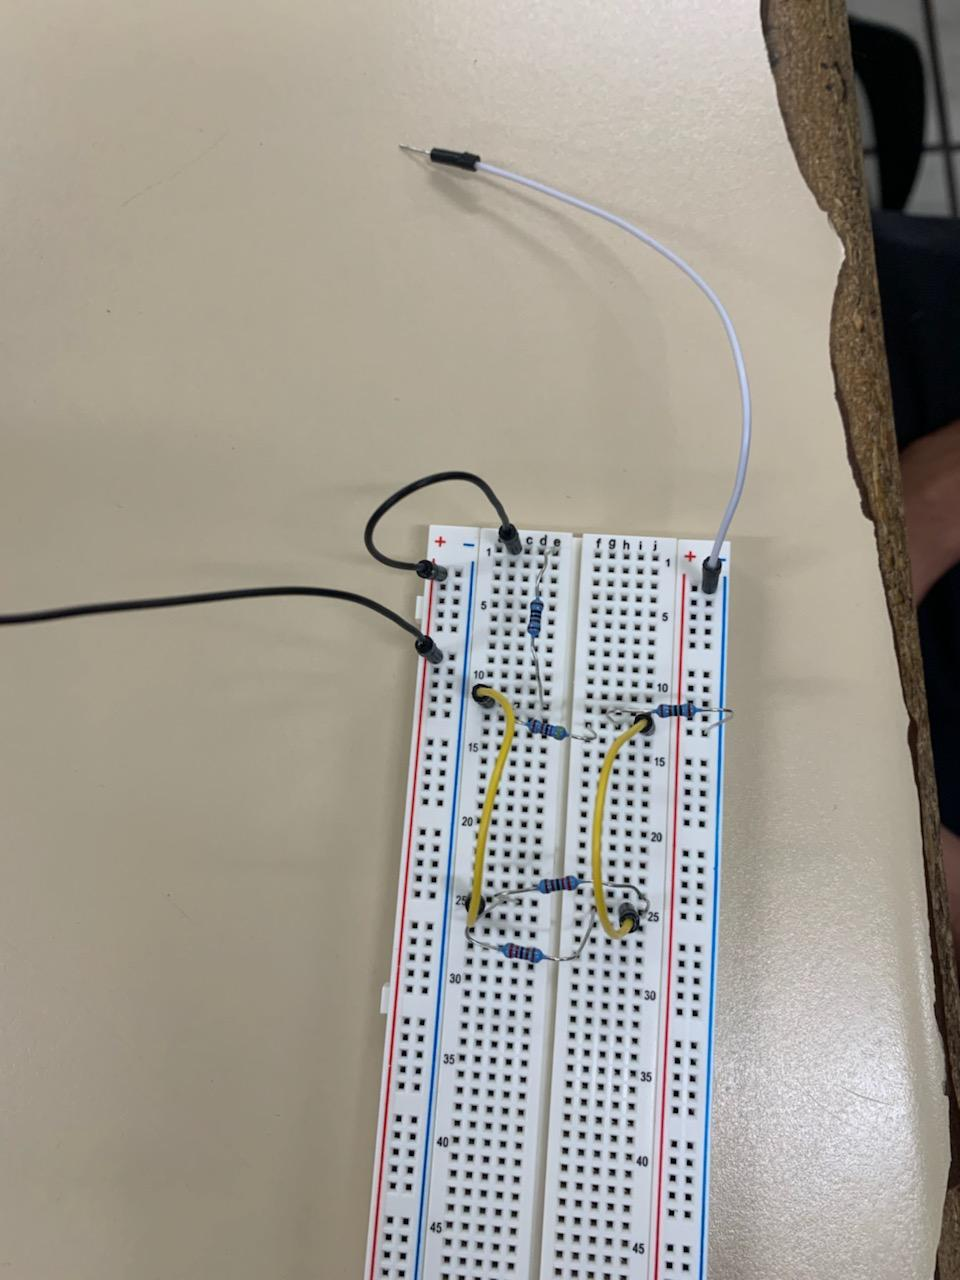
\includegraphics[width=\textwidth]{Breadboard.jpg}

\pagebreak

And here are all the values I tested for using a physical
digital multimeter:
\\
\\
\\
\begin{tabular}{r|l}
    $R_1$ & \SI{998}{\ohm}\\
    $R_2$ & \SI{4.7}{\kilo\ohm}\\
    $R_3$ & \SI{2.2}{\kilo\ohm}\\
    $R_4$ & \SI{2.2}{\kilo\ohm}\\
    $R_5$ & \SI{997}{\ohm}\\
    $I_T$ & \SI{3.11}{\milli\ampere}\\
    $I_1$ & \SI{0.60}{\milli\ampere}\\
    $I_2$ & \SI{1.25}{\milli\ampere}\\
    $I_3$ & \SI{1.25}{\milli\ampere}\\
    $I_4$ & \SI{3.11}{\milli\ampere}\\
    $V_{R_1}$ & \SI{3.11}{\volt}\\
    $V_{R_2}$ & \SI{2.77}{\volt}\\
    $V_{R_3}$ & \SI{2.77}{\volt}\\
    $V_{R_4}$ & \SI{2.77}{\volt}\\
    $V_{R_5}$ & \SI{3.11}{\volt}\\
\end{tabular}

\end{document}
